\begin{samplecase}
{\bf Different level density models : n + ${}^{99}$Tc}\newline
To demonstrate the variety of level density models that we have added 
recently to TALYS, we include a sample case in which 3 different models 
are compared. The results are given in Fig. \ref{tccum} for
the cumulative number of discrete levels and in Fig.\ref{tcnp} for the (n,p)
cross section.
\subsubsection{Case a: Constant Temperature Model}
The input file is

\VerbatimInput{\samples n-Tc099-ld1/org/talys.inp}

This is the default calculation: TALYS use the local CTM level density for
its calculations
\subsubsection{Case b: Back-shifted Fermi gas Model}
The input file is

\VerbatimInput{\samples n-Tc099-ld2/org/talys.inp}

\subsubsection{Case c: Hartree-Fock Model}
The input file is

\VerbatimInput{\samples n-Tc099-ld5/org/talys.inp}

\end{samplecase}
\begin{figure}
\centering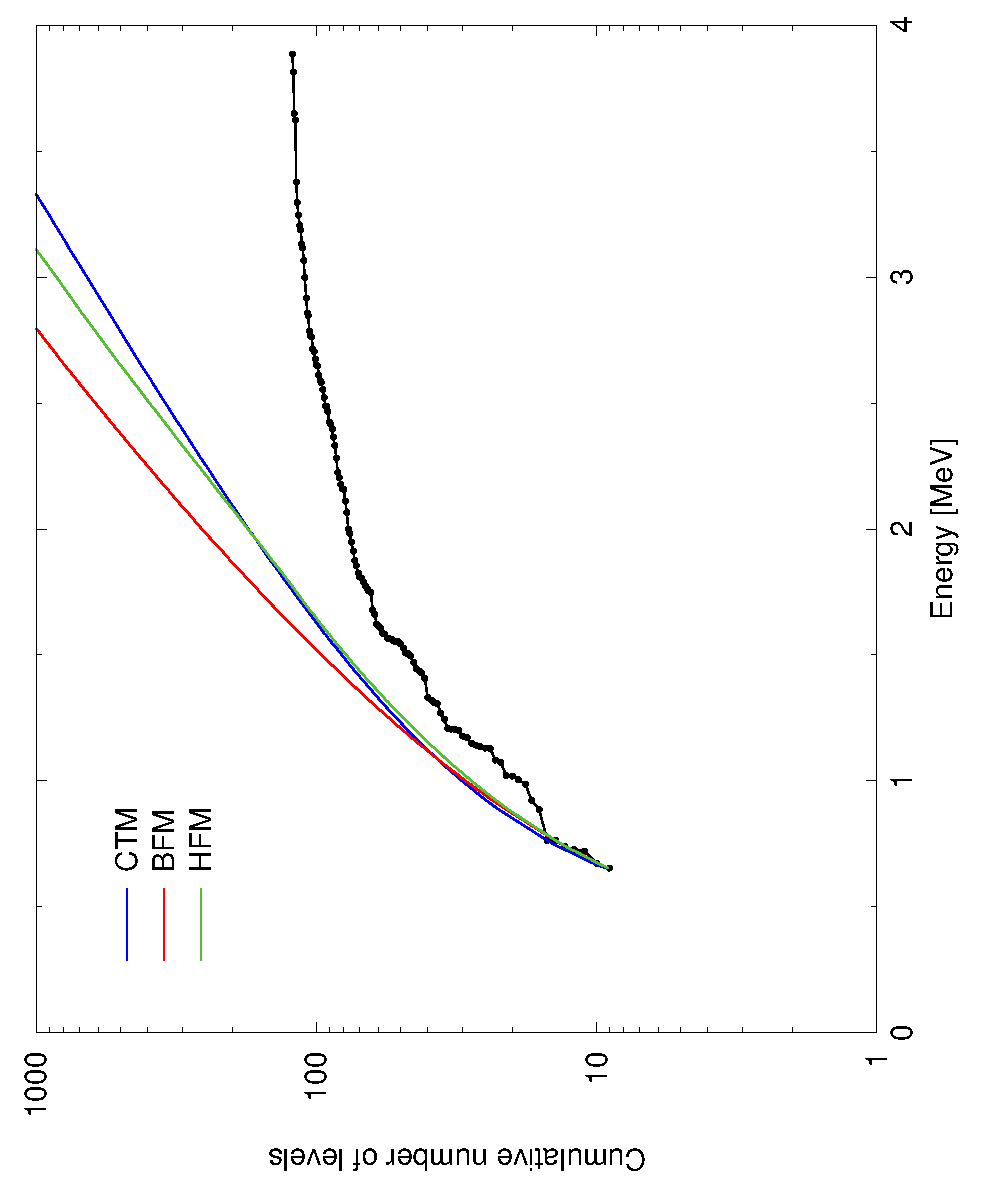
\includegraphics[scale=0.5,angle=270]{ldc}
\caption{Cumulative number of discrete levels of $^{99}$Tc for different 
level density models.}
\label{tccum}
\end{figure}
\begin{figure}
\centering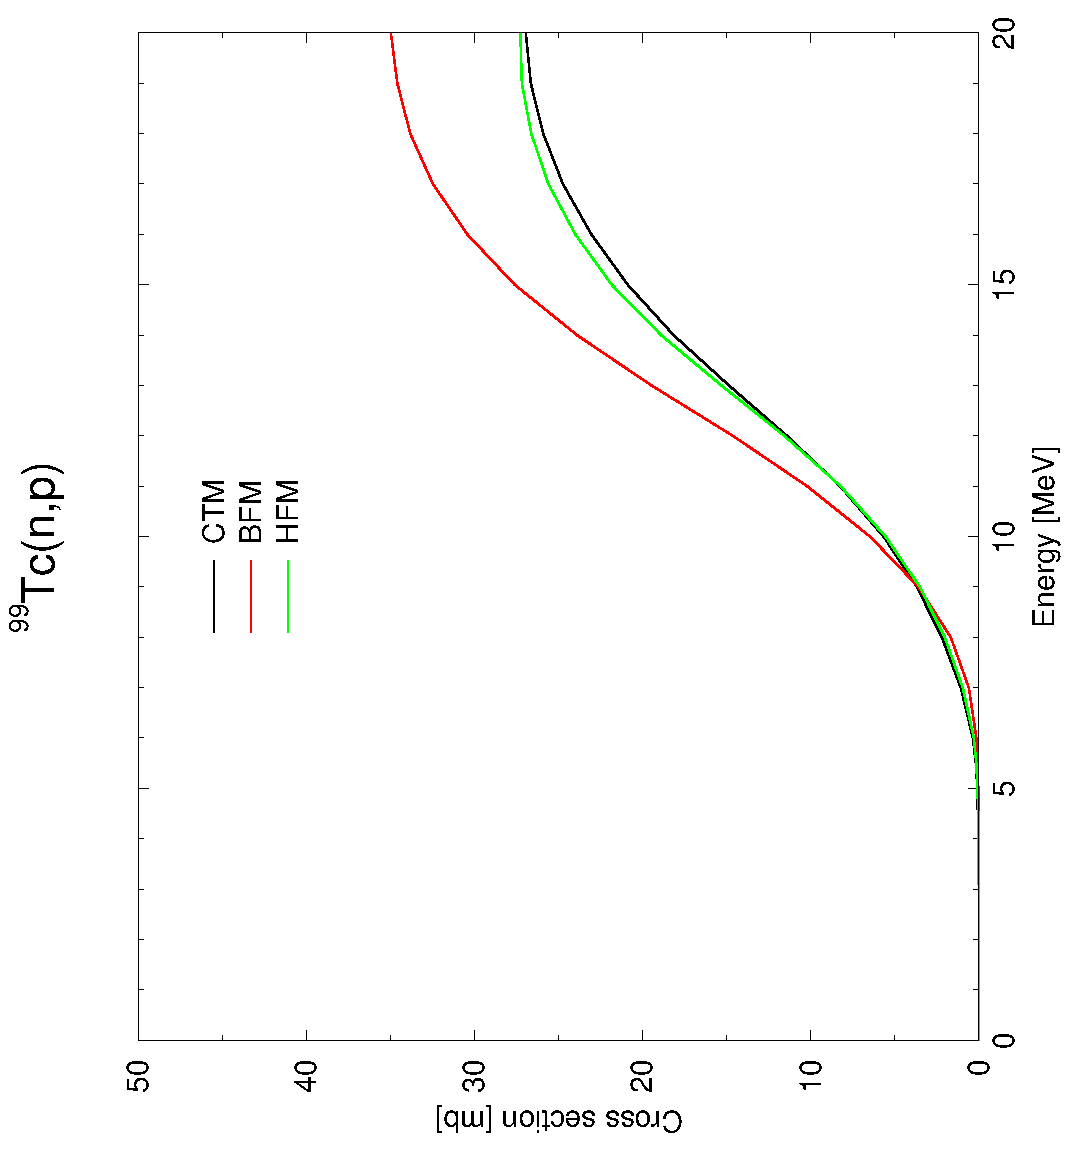
\includegraphics[scale=0.5,angle=270]{rp042099}
\caption{$^{99}$Tc(n,p) cross section for different 
level density models.}
\label{tcnp}
\end{figure}
